%%%%%%%%%%%%%%%%%%%%%%%%%%%%%%%%%%%%%%%%%%%%%%%%%%%%%%%%%%%
% --------------------------------------------------------
% RMxAA Rho
% LaTeX Template
% Version X.X.X (25/06/2025)
%
% Authors: 
% Carlos Román-Zúñiga (croman@astro.unam.mx)
% Irene Cruz-Gonzaélz )icruzgonzalez@astro.unam.mx)
% Contributors:
% Guillermo Jimenez (memo.notess1@gmail.com)
% Eduardo Gracidas (eduardo.gracidas29@gmail.com)
% 
% License:
% XXXXXXXXXX
% --------------------------------------------------------
%%%%%%%%%%%%%%%%%%%%%%%%%%%%%%%%%%%%%%%%%%%%%%%%%%%%%%%%%%%
% --------------------------------------------------------
%                     ACKNOWLEDGMENTS
% This template has been developed based on the original rho 
% LaTeX class work, created by Luis Guillermo Jimenez Lopez 
% and Eduardo Gracidas Reyes. Available in the Overleaf's 
% template gallery.
% --------------------------------------------------------
%%%%%%%%%%%%%%%%%%%%%%%%%%%%%%%%%%%%%%%%%%%%%%%%%%%%%%%%%%%
% The following lines must be included in all contributions
%
\documentclass[10pt,letter,twoside]{rmaa-rho-class/rmac-rho}
\RMxAAtemplatetype{\RMxAC} % Select your article type
% {\RMxAA} article template
% {\RMxAC} conference template

\newcommand\rmaatex{RMxAC~\LaTeX}
\newcommand{\CS}[1]{\texttt{\textbackslash #1}}
% Additional packages
\usepackage{background}
\usepackage{lipsum}
\definecolor{textcolor}{HTML}{F9C051}
%----------------------------------------------------------
% JOURNAL/HEADER INFORMATION
%----------------------------------------------------------

\vol{60}
% Counter page
\setcounter{page}{30}
\pages{30}
\thisyear{2026}

\doi{\href{https://www.astroscu.unam.mx/RMxAC/RMxAC..XX-X}{https://www.astroscu.unam.mx/RMxAC/RMxAC..XX-X}}


%\doi{ccccccccc}
\newenvironment{Example}
{\begin{list}{}{\setlength{\leftmargin}{10pt}\setlength{\rightmargin}{10pt}}%
  \item[]\itshape}
  {\end{list}}
%

% From here on the RMxAC extended article, onepage or only abstract information should be included by the author(s)
%
%----------------------------------------------------------
% TITLE
%----------------------------------------------------------
%\journalname{\Large Revista Mexicana de Astronomía y Astrofísica 62, 1-10 (2026) \hfill {\includegraphics[width=1.2in, height=0.5in]{LogoRMxACamarillo.png}} \\}

\title{Extended article for \rmaatex ~ template  v1.1}

%----------------------------------------------------------
% AUTHORS AND AFFILIATIONS
%---------------------------------------------------------

\author[1,$\dagger$]{Irene~Cruz-González \orcidlink{0000-0002-2653-1120}}
\author[2]{Carlos~G.~ Román-Zúñiga \orcidlink{0000-0001-8600-4798}}
\author[3,$\dagger$]{William~J.~Henney \orcidlink{0000-0001-6208-9109}}
%\author[1,2,$\dagger$]{A. Student}
%\author[2,4]{M.~Y.~Posdoc}

%----------------------------------------------------------

\affil[1]{Universidad Nacional Autónoma de México, Instituto de Astronomía, AP 106,  Ensenada 22800, BC, México}
\affil[2]{Universidad Nacional Autónoma de México, Instituto de Astronomía, AP 70-264, CDMX 04510, México}
\affil[3]{Universidad Nacional Autónoma de México, Instituto de Radioastronomía y Astrofísica.\\
Antigua Carretera a Pátzcuaro 8701, Ex-Hda. San José de la Huerta, 58089, Morelia, Michoacán, México}

%\affil[4]{One more affiliation you may need}
%\affil[$\dagger$]{This project is part of a collaboration/consortium/program}


%----------------------------------------------------------
% DATES
%----------------------------------------------------------

%\dates{This manuscript was compiled on June 25th, 2024}

%----------------------------------------------------------
% FOOTER INFORMATION
%----------------------------------------------------------

\leadauthor{Cruz-González et al.}



%----------------------------------------------------------
% Meeting details go here, that will appear in all the pages
%----------------------------------------------------------
\newcommand\Text{\small ``Local Volume Mapper III´', Zihuatanejo, Gro., Mexico, September 10-15, 2026.  \\~\\Volume Editors: Milky Way, Magellanic Cloud \& Messier 33}

\SetBgColor{textcolor}
\SetBgOpacity{1}
\SetBgAngle{90}
\SetBgPosition{current page.center}
\SetBgVshift{-0.46\textwidth}
%\SetBgVshift{-0.36\textwidth}
\SetBgScale{1.2}
%\SetBgScale{1.8}
\SetBgContents{\sffamily\Text}


%\institution{Universidad Nacional Autónoma de México}
%\footinfo{Creative Commons CC BY 4.0}
%\theday{November 20th, 2024} %\today

%----------------------------------------------------------
% ARTICLE INFORMATION
%----------------------------------------------------------

%\corres{icruzgonzalez@astro.unam.mx}
%\email{icruzgonzalez@astro.unam.mx}

\received{\today}
%\revised{April 16, 2024}
\accepted{\today}
%\published{May 21, 2024}
%\doi{\url{https://www.astroscu.unam.mx/rmaa/RMxAA..XX-X}}

%\license{Rho LaTeX Class \ccLogo\ This document is licensed under Creative Commons CC BY 4.0.}
%----------------------------------

%----------------------------------------------------------
% ABSTRACT
%----------------------------------------------------------
\setbool{rho-abstract}{true} % Set false to hide the abstract
\setbool{rho-resumen}{false} % Set false to hide the abstract
\corres{icruzgonzalez@astro.unam.mx}

\begin{abstract}
This file provides an example {\bf rmac\_onepage\_example.tex}  of the one page only articles for Revista Mexicana de Astronomía y Astrofísica Serie de Conferencias.  We refer authors to a brief tutorial of macros (V4.1 RMxAC \LaTeX{} macros) 
in the {\bf rmac\_extended\_example.tex} guide, and uses {rmac-rho.cls} template. It provides tutorial information and a common template for authors to prepare their conference proceedings contributions (extended, short, or abstract) for submission to the Special Editors of the corresponding volume of your meeting to appear in RMxAC. It is assumed that the author is already familiar with the rudiments of \LaTeX{}.  This file is  a template for the preparation of {\bf onepage} papers to be published in  RMxAC. 
\end{abstract}


%----------------------------------------------------------

\keywords{keyword 1, keyword 2, keyword 3, keyword 4, keyword 5}


%----------------------------------------------------------

\begin{document}
	
\maketitle
\pagestyle{fancy}
\thispagestyle{firststyle}

%corresponfing author
%\footnote{{\color{rhocolor} {\small \bf Corresponding author:}} {icruzgonzalez@astro.unam.mx}}
%\tableofcontents

%----------------------------------------------------------

\RMxAAstart{G}iven that you only have one page, you probably don't want to waste
space with frivolities, such as section headings.  The following text (from W.J. Henney paper) is just a typical short paper with equations, one figure, and a few references.

The general structure of the flow variables along the symmetry axis of the bowshock shell is illustrated schematically in Figure~\ref{fig:simple}.  The approximately isothermal proplyd flow accelerates from the sound speed to a Mach number $\mathcal{M}_0$ at the position of the shock. If the number density and temperature immediately before the shock are $N_0$, $T_0$, then the 
Rankine-Hugoniot conditions give the values immediately after the shock to be \citep{1987flme.book.....L}. %(Landau \& Lifschitz 1987)
%
% Equations are numbered
%
\begin{equation}
  \label{eq:mjump}
  \mathcal{M}_1 = \left( \frac{ \mathcal{M}_0^2 + 3 } { 5
      \mathcal{M}_0^2 - 1 } \right)^{1/2} , 
\end{equation}
\begin{equation}
  \label{eq:njump}
  N_1 = \frac{ 4 } { 1 + 3 \mathcal{M}_0^{-2} } N_0 , 
\end{equation}
\begin{equation}
  \label{eq:tjump}
  T_1 = \frac{1}{16} \left( 5 \mathcal{M}_0^2 - 1 \right) 
  \left( 1 + 3 \mathcal{M}_0^{-2} \right) T_0 .
\end{equation}

For instance, using $\mathcal{M}_0 = \mathcal{M}_{A} = 2.7$ from their equation~(99), one obtains $\mathcal{M}_1 = 0.54$,    $N_1 = 2.83 N_0 = 5.77 \times 10^4$\,cm$^{-3}$, $T_1 = 3.13 T_0 =30,500$ ,K, so that the density and temperature jump across the shock are both roughly a factor of 3.

%The emission from the cooling zone behind the shock can be crudely approximated as the emission from a homogeneous layer with density $N_1$ and temperature $T_1$ and with a width equal to the cooling time $t_{cool} = 3 k T_1 / \left( N_1 \Lambda_1 \right)$ multiplied by the immediate postshock velocity $v_1 = \mathcal{M}_1 (T_1/T_0)^{1/2} c_0 \simeq 11.5$\,km\,s$^{-1}$. 
To estimate the cooling coefficient $\Lambda_1$ in the cooling zone, we calculated another Cloudy model, identical to that mentioned above, except that the electron temperature was artificially maintained at $T_{e} = T_1$. The result was $\Lambda_1 = 4.46 \times 10^{-23}$\,erg\,cm$^{3}$\,s$^{-1}$, giving a cooling time $t_{cool} = 4.9 \times 10^6$\,s and a cooling zone thickness $h_{cool} = 5.64 \times 10^{12}$\,cm. Although the \ion{O}{3} optical lines are still significant coolants in the cooling zone (20\% of the total), they are now supplanted in importance by the \ion{C}{3} NUV (28\%) and FUV (26\%) lines.
%
%%%%% Figure 
%
\begin{figure}[!t]
\centering
  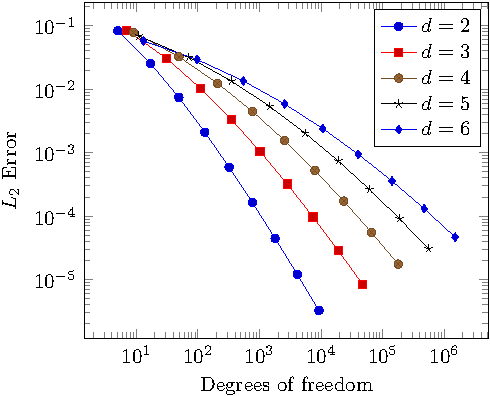
\includegraphics[width=0.90\columnwidth,height=4.0cm]{figures/example2.pdf}
  \caption{Example of a simple single-column figure. Don't put this
    too early in the document since we don't want it to go in the
    first column.}
  \label{fig:simple}
\end{figure}




%----------------------------------------------------------

\bibliography{rmxac}

%----------------------------------------------------------

\end{document}
 
        